\documentclass[12pt,a4paper,titlepage,final]{article}

% velikost stranky
\usepackage[top=2.5cm, left=2cm, text={17cm, 25cm}, ignorefoot]{geometry}

%%% ENCODING AND LANGUAGE
\usepackage[czech]{babel}
\usepackage[utf8]{inputenc}

%%% Hyperlinks
\usepackage[bookmarksopen,colorlinks,plainpages=false,urlcolor=blue,unicode,linkcolor=blue]{hyperref}
\usepackage{url}

%%% Tables
\usepackage{multirow}
\usepackage{booktabs}

%%% Figures
\usepackage{graphicx}

%%% Math
\usepackage{mathtools}
\usepackage{amsfonts}

%%%%%%%%%%%%%%%%%%%%%%%%%%%%%%%%%%%%%%%%%%%%%%%%%%
%%%%%%%%%%%%%%%%%%%%%%%%%%%%%%%%%%%%%%%%%%%%%%%%%%
%%%%%%%%%%%%%%%%%%%%%%%%%%%%%%%%%%%%%%%%%%%%%%%%%%
\begin{document}


\pagenumbering{arabic}
\setcounter{page}{1}

%%%%%%%%%%%%%%%%%%%%%%%%%%%%%%%%%%%%%%%%%%%%%%%%%%
%%%%%%%%%%%%%%%%%%%%%%%%%%%%%%%%%%%%%%%%%%%%%%%%%%
% title
    
\begin{centering}
\textsc{\textbf{PRL Paralelní a distribuované algoritmy} \\
FIT VUT Brno\\
}

\rule{\textwidth}{1.6pt}\vspace*{-\baselineskip}\vspace*{25pt} 

\begin{LARGE}
\textsc{Pipeline merge sort}
\end{LARGE}

\rule{\textwidth}{1.6pt}\\ % Thick horizontal line

\vspace*{5pt} 
\begin{footnotesize}
\today
\end{footnotesize}
\vspace*{5pt} 

\begin{large}
Jan Bednařík (xbedna45)\\
\end{large}

\end{centering}

%%%%%%%%%%%%%%%%%%%%%%%%%%%%%%%%%%%%%%%%%%%%%%%%%%
%%%%%%%%%%%%%%%%%%%%%%%%%%%%%%%%%%%%%%%%%%%%%%%%%%
% Obsah

%%%%%%%%%%%%%%%%%%%%%%%%%%%%%%%%%%%%%%%%%%%%%%%%%%
\section{Úvod}
V tomto dokumentu je popsána problematika řazení prvků pomocí algoritmu \texttt{Pipeline merge sort} na multiprocesorovém systému. Práce vznikla v rámci projektu v kurzu Paralelní a distribuované algoritmy (PRL), kdy bylo úkolem algoritmus implementovat v jazyce \texttt{C++} s použitím knihovny \texttt{OpenMPI} a experimentálně ověřit jeho předpokládanou časovou složitost.

%%%%%%%%%%%%%%%%%%%%%%%%%%%%%%%%%%%%%%%%%%%%%%%%%%
\section{Rozbor algoritmu}
Algoritmus staví na lineární topologii procesorů s tím, že vstupní data postupně proudí od procesoru s nižším pořadovým číslem k procesoru s vyšším pořadovým číslem ve formě \textit{zřetězené linky}. Každý procesor $P_i$ (kromě procesoru $P_0$) vytváří seřazenou posloupnost délky $2^i$ ze dvou příchozích seřazených posloupností délky $2^{(i-1)}$, disponuje tak dvěma frontami délky $2^{(i-1)}$. Nejprve plní příchozími daty první frontu, následně začne plnit druhou frontu a současně obě fronty řadit a posílat na výstup příslušné hodnoty. Procesor $P_0$ pouze čte vstupní data a posílá je procesoru $P_1$, tedy nepotřebuje žádnou vstupní frontu.

\paragraph{Časová složitost}
Procesor $S_i$ řadí dvě seřazené posloupnosti délky $d = 2^{(i-1)}$ a začne pracovat tehdy, jakmile od procesoru $S_{i-1}$ přijme první prvek (tedy jakmile procesor $S_{i-1}$ zapíše první prvek do své druhé fronty), což trvá $2d = 2*2^{i-1} = 2^{i}$ kroků. Vycházíme-li z předpokladu, že algoritmus běží na $P = log_{2}(N) + 1$ procesorech (kde $N$ odpovídá počtu řazených prvků), lze odvodit počet kroků $k$ nutných k zahájení řazení na posledním procesoru s pořadovým číslem $i = P - 1$.

\begin{equation}
k = 2^{i} = 2^{P - 1} = 2^{log_{2}(N)} = N
\end{equation}

Časová složitost algoritmu je tedy \textit{lineární}, $O(N)$.

\paragraph{Počet procesorů}
Počet kroků pro spuštění posledního procesoru, jenž má na výstupu seřazenou posloupnost, je $2^{P - 1}$, tedy lineární časové složitosti je dosaženo tehdy, je-li počet procesorů dán binárním logaritmem počtu vstupních prvků. K lineárnímu poli procesorů je přidán jeden další procesor, který čte vstupní posloupnost, tedy počet procesorů $P = log_2{N} + 1$

\paragraph{Paměťová složitost}
Procesor $i$ disponuje dvěma frontami délky $2^{(i-1)}$, tedy vyžaduje $2*2^{(i-1)} = 2^i$ paměťových jednotek. V případě posledního procesoru se jedná o celkem $N$ jednotek, v případě předposledního procesoru se jedná o $\frac{1}{2}N$ jednotek atd. Celkový počet paměťových jednotek dostaneme součtem této geometrické posloupnosti:

\begin{equation}
m = \frac{N}{1-\frac{1}{2}} = 2N
\end{equation}

Paměťová složitost je tedy \textit{lineární}, $O(N)$.

\paragraph{Cena}
Cena algoritmu je dána jako násobek počtu procesorů a časové složitosti, tedy $C(N) = N*log_2{N}$.

%%%%%%%%%%%%%%%%%%%%%%%%%%%%%%%%%%%%%%%%%%%%%%%%%%
\section{Implementace}
Program je implementován v \texttt{C++} s použitím knihovny \texttt{OpenMPI}, jež staví na zasílání zpráv mezi procesory. Komunikační protokol použitý pro implementaci algoritmu \textit{Pipeline merge sort} je znázorněný ve schématu \ref{fig:SequenceDiagram}. 

\begin{figure}[!hbt]
	\centering
	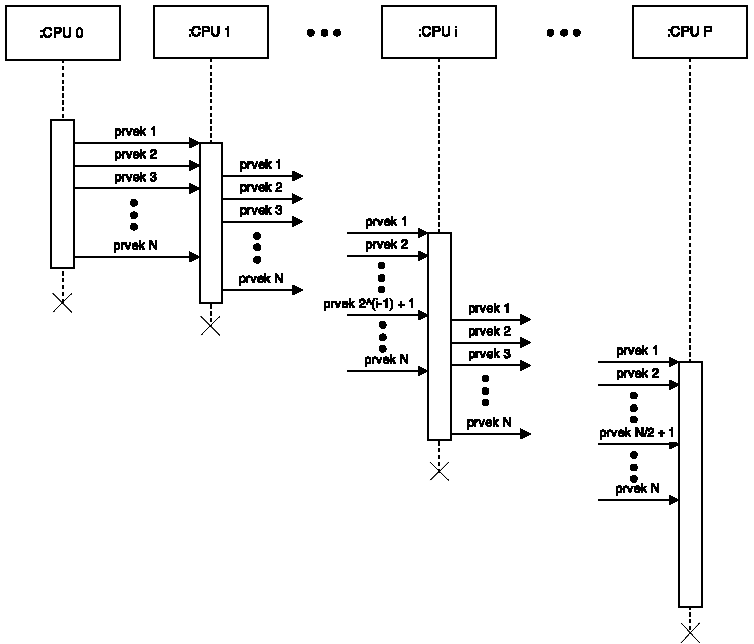
\includegraphics[width=1.0\linewidth]{img/sequence_diagram.pdf}
	\caption{Komunikační protokol procesorů vyjádřený sekvenčním diagramem pro obecný počet $N$ vstupních prvků a $P$ procesorů.}
	\label{fig:SequenceDiagram}
\end{figure}

Za účelem přehledné implementace byla oproti teoretickému odvození využita paměťová složitost dvojnásobná. Každému procesoru jsou namísto dvou front přiřazeny dvě dvojice front. Dokud procesor provádí řazení nad jednou dvojicí front, zapisuje se do druhé dvojice, a obráceně.

%%%%%%%%%%%%%%%%%%%%%%%%%%%%%%%%%%%%%%%%%%%%%%%%%%
\section{Experimenty}
Běh algoritmu byl otestován na referenčním serveru \texttt{merlin} vybaveným 6jádrovým CPU (12 vlákny). Testovány byly posloupnosti délky $N = 2^i, i \in \mathbb{N}, 10 \leq i \leq 20$, kde počet použitých procesorů $P = log_2{N} + 1$. Čas běhu staví na knihovní funkci \texttt{MPI::Wtime()} pro přesné měření času. Měření provádí pouze první procesor, kdy spouští časovač po načtení všech vstupních dat a před zasláním prvního prvku druhému procesoru. Jakmile poslední procesor zpracuje poslední hodnotu, zašle zprávu o dokončení řazení prvnímu procesoru, kterýžto po jejím přijetí zastaví časovač. Doba běhu tak není zatížena vstupně výstupními operacemi.

Testovací hardware musí fyzické procesory ve většině případů emulovat a testy byly navíc prováděny za běžného provozu serveru. Pro dosažení co nejvěrnějších výsledků tak byl pro každou délku posloupnosti $N$ test proveden desetkrát, z výsledků byly odstraněny dvě nejnižší a tři nejvyšší hodnoty a zbylých pět hodnot bylo průměrováno.

S použitím logaritmického měřítka časové osy a s ohledem na teoretickou časovou složitost $O(N)$ je očekáván lineární průběh závislosti doby běhu programu na počtu vstupních hodnot. Jak je patrné z grafu \ref{fig:CasVSPocetPrvku}, přes nepřesnosti způsobené nerovnoměrným vytížením testovacího stroje je závislost doby běhu na čase vskutku lineární.

\begin{figure}[!hbt]
	\centering
	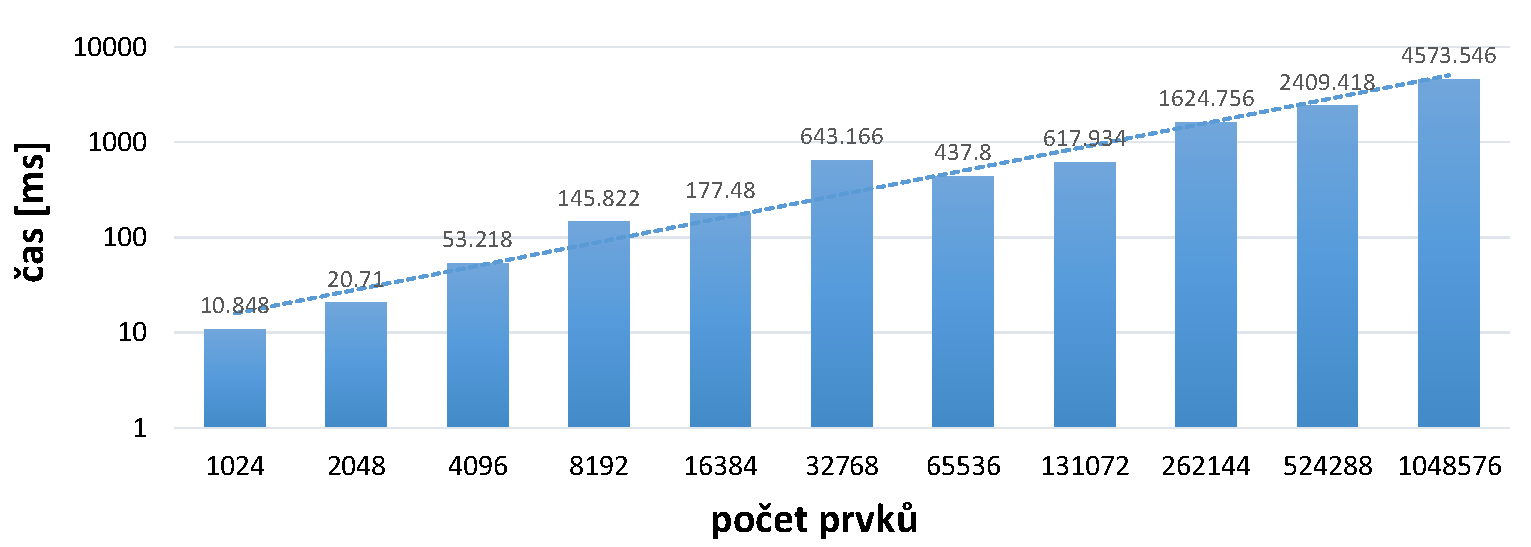
\includegraphics[width=1.0\linewidth]{img/time.pdf}
	\caption{Závislost doby běhu programu na počtu vstupních prvků.}
	\label{fig:CasVSPocetPrvku}
\end{figure}

%%%%%%%%%%%%%%%%%%%%%%%%%%%%%%%%%%%%%%%%%%%%%%%%%%
\section{Závěr}
V rámci projektu byl implementován algoritmus \textit{Pipeline merge sort}, byla odvozena jeho teoretická časová a paměťová složitost i cena a provedeny experimenty nad reálnými daty. Testy potvrdily lineární časovou složitost algoritmu, přesto byly zaznamenány nezanedbatelné odchylky. Ty jsou způsobené především proto, že testovací stroj nedisponuje dostatečným počtem procesorů (jader procesoru), tedy jednotlivé procesory požadované algoritmem jsou nahrazeny procesy sdílejícími výpočetní prostředky a neběží tak zcela paralelně. Testování bylo navíc prováděno za běžného provozu testovacího stroje, tudíž jsou výsledky ovlivněny aktuálními výpočetními požadavky ostatních uživatelů.

%%%%%%%%%%%%%%%%%%%%%%%%%%%%%%%%%%%%%%%%%%%%%%%%%%


\end{document}
